%
% File acl2015.tex
%
% Contact: car@ir.hit.edu.cn, gdzhou@suda.edu.cn
%%
%% Based on the style files for ACL-2014, which were, in turn,
%% Based on the style files for ACL-2013, which were, in turn,
%% Based on the style files for ACL-2012, which were, in turn,
%% based on the style files for ACL-2011, which were, in turn, 
%% based on the style files for ACL-2010, which were, in turn, 
%% based on the style files for ACL-IJCNLP-2009, which were, in turn,
%% based on the style files for EACL-2009 and IJCNLP-2008...

%% Based on the style files for EACL 2006 by 
%%e.agirre@ehu.es or Sergi.Balari@uab.es
%% and that of ACL 08 by Joakim Nivre and Noah Smith

\documentclass[11pt]{article}
\usepackage{acl2015}
\usepackage{times}
\usepackage{url}
\usepackage{latexsym}
\usepackage{amsmath}
\usepackage{graphicx}
\usepackage{amssymb}

%\setlength\titlebox{5cm}

% You can expand the titlebox if you need extra space
% to show all the authors. Please do not make the titlebox
% smaller than 5cm (the original size); we will check this
% in the camera-ready version and ask you to change it back.


\title{Exploring and Visualizing the Limitations of State-of-the-Art Graph Neural Networks with Long-Range Interactions}

\author{Alison Camille Dunning \\
  Halıcıoğlu Data Science Institute, UC San Diego / La Jolla, CA \\
  {\tt adunning@ucsd.edu}}

\date{}

\begin{document}
\maketitle
\begin{abstract}
    Graph Neural Networks (GNNs) have become an increasingly popular method in machine learning tasks in non-Euclidean domains, where data are represented as graphs containing complex interdependencies. GNNs can effectively exploit these interactions to solve problems including classification, recommendation, and node property prediction, nullifying the assumption of Euclidean deep learning that instances are independent of each other. This report provides a brief survey and details the implementation and benchmarking, using PyTorch Geometric and PyTorch Lightning, of three foundational GNN architectures: Graph Convolutional Network (GCN), Graph Attention Network (GAT), and Graph Isomorphism Network (GIN), as well as the message-passing paradigm they follow. Beyond  the theoretical underpinnings of these architectures, this report attempts to quantify and visualize their difficulties with capturing long-range dependencies (as well as maintaining short-term ones). Finally, it investigates a simplified graph rewiring mechanism, drawing inspiration from curvature-based approaches, to mitigate scaling issues in GNNS caused by oversquashing and information bottlenecks. The codebase for this report is available at \url{https://github.com/camille-004/gnn}.
\end{abstract}

\section{Introduction}

Underlying the breakthroughs of artificial neural networks are their capabilities in learning from rich, high-dimensional feature sets \cite{article}, synthesizing complex non-linear functions, and flexible mappings from one vector space to another. These make ANNs most successful in picking up hidden patterns within input data in a Euclidean domain. For example, convolutional neural networks (CNNs), which employ local connections and shift-invariance, are leveraged in numerous image analysis tasks to extract meaningful latent representations from images, which are expressed as grids in Euclidean space. However, applications of non-Euclidean datasets rapidly developing in the machine learning space. These include molecular fingerprints \cite{https://doi.org/10.48550/arxiv.1509.09292}, community detection \cite{9722614}, and recommendation systems \cite{https://doi.org/10.48550/arxiv.2109.12843}, and any other complex system of interactions that can be abstracted by a graph structure. Graph datasets pose challenges of different unordered node sets, edge and node weighting, and variable size node neighborhoods. As such, as deep learning approaches continue to extend to the irregularities within graph data, operations, such as convolution and attention, that have been exploited by traditional deep learning frameworks must become generalized.


\subsection{Message-Passing Architectures}
The problem of \textit{geometric deep learning} \cite{https://doi.org/10.48550/arxiv.2104.13478} has culminated in the invention of graph neural networks (GNNs). This report hones in on the following fundamental GNN variants: Graph Convolutional Network (GCN) \cite{https://doi.org/10.48550/arxiv.1609.02907}, Graph Attention Network (GAT) \cite{https://doi.org/10.48550/arxiv.1710.10903}, and Graph Isomorphism Network (GIN) \cite{xu2018how}. The particular class of GCN this report explores is the Fast Approximation Spectral-Based Graph Convolutional Neural Network proposed by Kipf and Welling. Intuitively, the Spectral GCN is a signal propagation along nodes, using the Eigen-decomposition of the graph Laplacian matrix, $\mathcal{L}$, to infer the structure of the graph. The graph Laplacian encodes the adjacency matrix, $A$, which is taken into account by the Fast Approximation method. The forward propagation equation includes $A$ as well as node features, so that the model learns features based on node connectivity, and it is then fed into a non-linear activation function \cite{8436869} to represent the features in a latent dimension. Additionally, a renormalization scheme is introduced to mitigate vanishing gradients. GATs capitalize on localization, computing unnormalized coefficients, $e_{ij}$, across pairs of nodes $i$ and $j$ based on their features (in addition to the crude structure of the graph). GINs have an empirical discriminative power advantage compared to GCNs, and are analogous to the Weisfeiler-Lehman test for graph isomorphism \cite{https://doi.org/10.48550/arxiv.1101.5211}. 


The message-passing paradigm, of which the convolutional and attentional flavors of GNN can be seen as special cases, fundamentally falter in capturing long-range interactions, i.e., information exchange between distant nodes \cite{https://doi.org/10.48550/arxiv.2206.08164}. The message-passing neural network (MPNN) propagation scheme \cite{https://doi.org/10.48550/arxiv.1704.01212} is as follows:

\begin{enumerate}
    \item Each node $i$ synchronously computes a “message"---a function $\phi(x_i, x_j, e_{ij})$, $j\in\mathcal{N}(i)$---for its first-order (one-hop) neighborhood $\mathcal{N}(i)$. $e_{ij}$ is some edge attribute.
    \item The nodes aggregate the messages they receive, using some permutation-invariant function  $\square_{j\in\mathcal{N}(i)}$---often a sum or average.
    \item Finally, each node performs on itself a feature representation update $\gamma$ that depends on the aggregated messages and its current attributes.
\end{enumerate}

Notationally,
\begin{equation}
    x_i'=\gamma(x_i, \square_{j\in\mathcal{N}(i)}\phi(x_i, x_j, e_{ij}))
\end{equation}

\subsection{Shortcomings with Long-Term Dependencies}

The order of the neighborhood can be increased for tasks requiring long-range information propagation. An MPNN can stack $L$ layers to encode information from an $L$-th order neighborhood. This causes the receptive field, $B_L(i)$ of each node to grow exponentially with $L$, bringing about an \textit{information bottleneck}, and an \textit{over-squashing} of an overload of information into fixed-size vectors \cite{https://doi.org/10.48550/arxiv.2006.05205}. Recent papers remark the drops in discriminative power in tasks that rely propagation between nodes, rather than local structural information. Propagating messages across non-adjacent nodes in a network without distorting them is an ongoing challenge in graph learning problems.

Alon and Yahav also propose using a fully-connected graph at the final layer \cite{https://doi.org/10.48550/arxiv.2006.05205} to "enforce" node connections that would've otherwise been squashed by the bottleneck, an approach that was consequently embraced by works in Graph Transformers \cite{NEURIPS2021_b4fd1d2c}. Additionally, Topping et. al. (2021) establish an intuitive formalization of the oversquashing effect, using the Jacobian of node representations to express gradient flows between adjacent and non-adjacent nodes under differentiable conditions. This report visualizes the distributions of Jacobian "influence scores" between a fixed node and each node in its $r$-hop neighborhood, for $r=1,...,10$.   

On the other hand, \textit{oversmoothing} arises from the Laplacian smoothing \cite{https://doi.org/10.48550/arxiv.1801.07606} of graph convolution operators on node features and graph topology. Laplacian smoothing effectively strengthens similarities among nodes in the same cluster, but with more convolutional layers, differences between output representations may become indiscernible. mall datasets are especially susceptible to this, as shown in the results portion of this report. The Dirichlet energy of embeddings \cite{https://doi.org/10.48550/arxiv.2006.13318} as a function of the GNN layer ID is used to visualize the loss of discriminative power. Cai and Wang (2020) also briefly mention the Rayleigh quotient (normalized Dirichlet energy) to quantify real oversmoothing effects. As a possible remedy, Li et. al. (2018) introduced training a random walk model in tandem with a self-training GCN to explore global graph topology. This is applied to the semi-supervised graph learning problem, which employs graph/manifold structure to learn with a limited amount of labels. 

\subsection{Graph Rewiring}

Graph rewiring produces a new graph, $\mathcal{G}'' = (\mathcal{V}, \mathcal{E}')$ with a different edge structure. Topping et. al. outline the procedure as a corrective to the information bottleneck, and they propose a rewiring scheme that evolves negative curvature without undermining the statistical properties of the input graph. For exploration, this experiment in this report rewires the input graphs by simply adding random edges, the amount of which is determined by a threshold expressed as a percentage of the original number of edges. As this method does not account for topology, the information-to-noise ratio in the graph is lowered, thus reducing the performances of the networks as the threshold increases, contrasting from the results of Topping et. al.

\begin{figure}
    \centering
    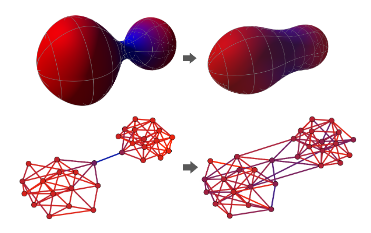
\includegraphics[scale=0.5]{curvature.png}
    \caption{Adding a top evolution to the negative curvature, shown in blue, via edges, reduces the information bottleneck and oversquashing effect. From \textit{Understanding over-squashing and bottlenecks on graphs via curvature}, by Topping et. al., 2021, ICLR 2022.}
    \label{fig:curvature}
\end{figure}

The goals of this report are twofold:
\begin{itemize}
    \item Obtain Dirichlet energy and Rayleigh quotient values for each layer in baseline a MPNN with a variable number of hidden layers, and determine whether they always converge to zero after passing through layers. This is observed more consistently with the Rayleigh quotient. Also, after training each network, plot the $r$-hop neighborhood influence distributions on a fixed node.   
    \item Perform a randomized graph rewiring scheme and observe the MPNN performance with different amounts of edges added. On the particular homophily node classification datasets used, a drop in performance with adding more edges is observed, which could be attributed to oversmoothing, a decreased information-to-noise ratio, and a lack of long-range interactions.
\end{itemize}

\section{Preliminaries and Notation}

Define a graph as a pair $\mathcal{G}=(\mathcal{V}, \mathcal{E})$, comprising a vertex set $\mathcal{V}$, with $|\mathcal{V}|=n$ and an edge set $\mathcal{E}$. Denote the non-negative matrix $A=[a_{ij}] \in \mathbb{R}^{n \times n}$. $D=\text{diag}(d_1,d_2,...,d_n)$, where $d_i=\sum_j a_{ij}$ is the degree matrix, and the graph Laplacian is defined as $L := D-A$, where $L$ can be normalized, such as $\tilde{L}=I-D^{-\frac{1}{2}}AD^{-\frac{1}{2}}$. In graph learning, we consider a graph $\mathcal{G}=(\mathcal{V}, \mathcal{E}, X)$, where $X=[x_1,x_2,...,x_n]^\top \in \mathbb{R}^{n \times d}$, and $x_i \in \mathbb{R}^d$ is a feature vector of node $i$. This paper focuses only on the downstream task of node classification (either supervised or semi-supervised) on homophily graphs. The targets are node properties and the inputs are the embedding vectors and the adjacency matrix of the graph. 

\subsection{Architecture Definitions}

\subsubsection{Graph Convolutional Network}

Graph convolutional neural networks use either spatial-based \cite{https://doi.org/10.48550/arxiv.1909.05310} or spectral-based \cite{https://doi.org/10.48550/arxiv.1609.02907} methods. This report concentrates only on the latter, particularly the fast approximate convolutions on graphs presented by Kipf and Welling (2017). The layer-wise propagation rule is as follows:

\begin{equation}
    H^{(l + 1)} = \sigma \left(D^{-\frac{1}{2}}\tilde{A}D^{-\frac{1}{2}}H^{(l)}W^{(l)} \right)
\end{equation}

$\tilde{A} = A + I_N$ is the adjacency matrix of the undirected graph $\mathcal{G}$ with self-loops. A spectral convolution on a graph is the multiplication of a signal $x \in \mathbb{R}^n$ with a Fourier-domain filter $g_\theta$. The final spectral convolution is defined in this work as

\begin{equation}
    g_\theta' \star x \approx \sum_{k=0}^{K} \theta_k'T_k(\tilde{L})x
\end{equation}

$\tilde{L}$ is a rescaled normalized graph Laplacian, $T_k$ is the recursive relation defining the Chebyshev polynomials, and the expansion of the Chebyshev polynomials up to the $K$-th order is suggested by Hammond et. al. (2009) \cite{https://doi.org/10.48550/arxiv.0912.3848} to approximate $g_\theta(\Lambda)$, where $\Lambda$ is the diagonal matrix of the eigenvalues of $L$. The GCN stacks convolutional layers, each followed by a non-linearity. Free parameters are limited to constrain eigenvalues, and a renormalization trick on the adjacency matrix, the notation of which is presented in the original work, to alleviate vanishing gradients. (In this report's implementation, non-linearities were only kept after the first and last convolutional layers, to experiment with the network performance metrics.)  

\subsubsection{Graph Attention Network}

GATs exploit the attention technique \cite{https://doi.org/10.48550/arxiv.1710.10903} to assign different weights to different neighboring nodes. $\alpha_{vu}$ is a weighting factor of a node $u$'s message to node $v$. We can define $\alpha$ based on the graph structure, instead of using an average aggregation, $\alpha_{vu}=\frac{1}{\mathcal{N}(v)}$. Calculate attention coefficients $e_{vu}$ across the pairs of nodes $u$, $v$, with any attention mechanism $a$, (whose parameters can be trained jointly with $W_k$) as follows:

\begin{equation}
    e_{vu} = a(W_kh_u^{k-1},W_kh_v^{k-1})
\end{equation}

The attention coefficient specifies the importance of the message from node $u$ to node $v$. Then, to compare the importance across different neighbors, the coefficients are normalized using softmax:

\begin{equation}
    \alpha_{vu}=\frac{\text{exp}(e_{vu})}{\sum_{k \in \mathcal{N}(v)}\text{exp}(e_{vk})}
\end{equation}

Finally, the resulting embedding becomes:

\begin{equation}
    h_v^k = \sigma \left( \sum_{u \in \mathcal{N}(v)} \alpha_{vu}W_kh_u^{k-1} \right)
\end{equation}

In Alon and Yahav's empirical observation of the bottleneck, GAT was less susceptible to over-squashing than GIN and GCN, since GAT's attention mechanism weighs incoming messages such that irrelevant edges are ignored by the target node. This report verifies this in the results.

\subsubsection{Graph Isomorphism Network}

The graph isomorphism network's aggregator is designed to discriminate graphs. As such, owing to its high expressive power, it achieves higher accuracy on graph classification tasks than does the GCN. However, it performs less adequately when expressive power is more dispensable, i.e., with rich feature-sets in node classification tasks. The authors of GIN suggest using the Weisfeiler-Lehman test for graph isomorphism \cite{xu2018how} as a heuristic to characterize the "representational power" of GNNs. Graph isomorphism occurs when two graphs have the same connections but different permutations of nodes. As graph discrimination might be an NP-intermediate computationally complex task and isn't known to be solvable in polynomial time, isomorphism isn't guaranteed by the Weisfeiler-Lehman test, but non-isomorphism can be detected. Identified by researchers to be analogous to how GNNs learn, the Weisfeiler-Lehman test proceeds as follows:

\begin{enumerate}
    \item Each node has an identical label.
    \item Neighbors are aggregated and hashed to produce a new label.
    \item Repeat until the labels stop changing.
\end{enumerate}

Xu et. al. (2019) use multi-layer perceptrons (MLPs) to learn two injective functions, $f$ and $\phi$ for neighbor aggregation, since, from Theorem 3 in their work, if neighbor aggregation (and graph-level readouts) are injective, then the resulting GNN is as powerful as the Weisfeiler-Lehman test. The authors invent an aggregator that should produce different node embeddings for non-isomorphic graphs, provided these conditions hold. With $\epsilon$ as either a learnable parameter or fixed scalar, GIN updates node representations as:

\begin{equation}
    h_v^{(k)} = \text{MLP}^{(k)} \left(\left(1 + \epsilon^{(k)}\right) \cdot h_v^{(k - 1)} + \sum_{u \in \mathcal{N}(v)} h_u^{(k - 1)}\right)
\end{equation}

\subsection{Oversquashing}

This subsection defines the metrics gathered in this report to gauge oversquashing.

\subsubsection{Jacobian Influence Score}
Define $d_G$ as the standard shortest-path distance on the graph. Given $i\in \mathcal{V}$, let

\begin{equation}
    S_r(i):={j\in \mathcal{V} : d_G(i, j)=r}, r \in \mathbb{N}
\end{equation}

Assume a hidden feature $h_i^{(\ell)}$ is a differentiable function computed by an $\ell$-layer MPNN of node features ${x_1,...,x_n}$, and update and message functions $\phi_{\ell}$ and $\psi_{\ell}$ are differentiable. As over-squashing can be expressed in terms of one node representation $h_i^{(\ell)}$ failing to be affected by some input feature $x_s$ of node $s$ at distance $r$ from node $i$, due to distortion (from vanishing gradients, composed aggregations, etc.), the Jacobian of node representations with respect to $x_s$ can be used to assess and quantify this effect \cite{https://doi.org/10.48550/arxiv.2111.14522}. 

\begin{equation}
    \left| \frac{\partial h^{(r + 1)_i}}{\partial x_s} \right|, s \in S_{r+1}(i)
\end{equation}

\subsection{Oversmoothing}

This subsection defines the metrics gathered in this report to gauge oversmoothing. 

\subsubsection{Dirichlet Energy}

The Dirichlet energy is based on measuring node pair differences. Consequently, it should converge to zero with increasing layers, as node emeddings become close together \cite{https://doi.org/10.48550/arxiv.2107.02392}. Works have even been devised to jointly optimize the task loss and energy value. Given a node embedding matrix $X^{(\ell)}=[x_1^{(\ell)}, x_2^{(\ell)}, ..., x_n^{(\ell)}]^\top \in \mathbb{R}^{n\times d}$ learned from the $\ell$-th layer, and a symmetric Laplacian matrix $L \in \mathbb{R}^{n\times n}$ of a graph $\mathcal{G}$, the Dirichlet energy $E(X^{(\ell)})$ is given by:

\begin{equation}
    \begin{aligned}
        E(X^{(\ell)}) &= \text{tr}(X^{(\ell)}^\top L X^{(\ell)}) \\
        & = \frac{1}{2}\sum a_{ij} \left\|  \frac{x_i^{(\ell)}}{\sqrt{1 + d_i}} - \frac{x_j^{(\ell)}}{\sqrt{1 + d_j}} \right\|
    \end{aligned}
\end{equation}

$a_{ij}$ is the edge weight, the $(i,j)$-th element in the adjacency matrix $A$, and $d_i$ is the node degree, the $i$-th element in the diagonal matrix $D$.

\subsubsection{Rayleigh Quotient}

Given a symmetric Laplacian matrix $L \in \mathbb{R}^{n\times n}$ of a graph $\mathcal{G}$, the Rayleigh quotient $R(L, f)$ for $f \in \mathbb{R}^n$ is given as:

\begin{equation}
    R(L, f) = \frac{f^\top Lf}{f^\top f} = \frac{1}{f^\top f}\sum_{u\sim v} (f(u) - f(v))^2
\end{equation}

\section{Evaluation} 

\subsection{Experimental Setup}

This experiment runs a suite of node classification tasks using baseline implementations of the three message-passing architectures. The training is full-batch, and the dimension of the hidden channels in the convolutional layers is 16. All networks except GAT use dropout after each layer\footnote{The removal of dropout layers from GAT seems to be a remnant from initial experimentation. For future work, dropout layers with equal probabilities should be reintroduced for all networks in the experiment, for a more reliable results comparison.}. Regardless, GAT retains its performative advantage to GCN and GIN, whether or not all models are using dropout. The GCN and GIN use a ReLU\footnote{As ReLU is non-differentiable, backwards calculations of the Jacobians might yield inaccurate values. For future work, a hyperbolic tangent activation should be used for the GCN and GIN instead.} activation function, and the GAT uses an ELU. The experiment is run on the following variables, resulting in a total of 192 models:

\begin{table}[h]
\begin{center}
\begin{tabular}{|l|rl|}
\hline \bf Variable & \bf Values & \\ \hline
add\_edges\_thres & 0.0, 0.2, 0.4, 0.6 & \\
model & GIN, GAT, GCN & \\
dataset & pubmed, citeseer, cora & \\
n\_hidden\_layers & 1, 2, 5, 10 & \\
n\_heads & 1, 16 (GAT only) & \\
\hline
\end{tabular}
\end{center}
\caption{\label{font-table} Parameters of the experiment and their possible values.  }
\end{table}

As only baseline models are tested, no hyperparameter optimization was performed. Future directions might also take into consideration the effect of methods such as batch normalization on the training process. For all networks, on each layer propagation, Dirichlet energy and Rayleigh quotient values are recorded. After training the networks, a random node is fixed, after which the Jacobians for that node's $r$-hop neighborhood, for $r=1,...,10$, are calculated via a backward pass.

\subsection{Datasets}

The "Citeseer", "Cora", and "Pubmed" datasets come from "Revisiting Semi-Supervised Learning with Graph Embeddings" \cite{https://doi.org/10.48550/arxiv.1603.08861}. In each of these graphs, the nodes represent documents and the edges are citation links.

\begin{table}[h]
\begin{center}
\begin{tabular}{|l|rrrr|}
\hline \bf Dataset & \bf Nodes & \bf Edges & \bf Feats. & \bf Classes & \hline
Citeseer & 3,327 & 9,104 & 3,703 & 6 &
Cora & 2,708 & 10,556 & 1,433 & 7 &
Pubmed & 19,717 & 88,648 & 500 & 3 &
\hline
\end{tabular}
\end{center}
\caption{\label{font-table} Dataset statistics. }
\end{table}

For this experiment, an 80/10/10 is carried out on each dataset.

\subsection{Limitations}

The use of the citation link datasets for this experiment poses limitations insofar as they aren't adopted in benchmarks for long-range interdependency tasks. Furthermore, the datasets are small compared to ones proposed in the Long Range Graph Benchmark \cite{https://doi.org/10.48550/arxiv.2206.08164}, which comprise tens of thousands of graphs with millions of nodes. Those datasets were not utilized in this experiment due to constraints with compute resources and time. Additionally, the baseline models have not been fully tuned to adapt to those used in other works, so the performance metrics haven't been successfully reproduced and are significantly lower, except perhaps with the GAT. In the high-homophily settings of the citation networks, methods, such as GAT and GCN, that favor local information, empirically achieve higher performance than more sophisticated ones. The citation networks can be resampled to become more suitable for prediction tasks utilizing information from farther nodes \cite{https://doi.org/10.48550/arxiv.2107.07432}. Rampášek and Wolf (2021) resample the citation link datasets such that a node's $k$th-order neighborhood is cleansed of labels, preventing the network from exploiting too much local information. Additionally, the experiment could consider models with no hidden layers (i.e., convolution layers with dimensions (\textit{hidden\_dim}, \textit{hidden\_dim})), and only the input and output convolution layers. Finally, there are no available works that visualize the Dirichlet energy, Rayleigh quotient, and node representation Jacobian values in this experimental setting, so the correctness of the resulting plots are difficult to gauge.  


\section{Results}

This section will consider the experimental results only for the PubMed dataset. The reader is referred to the report's affiliated GitHub repository, which stores the rest of the generated figures.

\subsection{Effect of Adding Random Edges and Layers on Performance Metrics}

For the original input graph and with a small amount of data augmentation, the results of both the single-head and multi-head GAT well outperform the GCN and GIN (Figure A\ref{fig:performance}). GATs may also employ multi-head attention, which is analogous to multiple channels in a convolutional network. Although multi-head attention is designed to enhance model capacity and stabilize learning, both the validation and test accuracy demonstrate the oversquashing pitfall of the increased model complexity. The drop in performance as the number of hidden layers increases is noticeable, even relative to that of the GCN and GIN. The GIN's accuracies actually increase until the number of hidden layers reaches 10, although this is not enough to renounce the empirical predisposition of GINs to oversquashing, as the metrics still average to around 35 percent. The same holds for the GCN, although the accuracy trends fluctuate much more. From Figure A\ref{fig:performance}, with the exception of the GCN, the random addition of a larger amount of yields a much less performant network. The oversquashing effects are more visually apparent with the GATs, but because the overall accuracies are much higher, this result still verifies that these networks are less vulnerable to oversquashing than their MPNN counterparts.

\subsection{Oversquashing Metrics}

After training of the network, the Jacobian of the embedding of neighbors at a distance $r$ from a fixed node $s$, with respect to the features of $s$, is calculated via a backward pass. The indices of the nodes within the $s$'s $r$-hop neighborhood are used to identify the correct rows in the Jacobian matrix. For each neighboring node, the vectors from the Jacboian are summed, resulting in a distribution of "influence" scores on $s$ of the $r$-hop neighborhood. This is done for $r=1,...,10$, resulting in ten different distributions for different-order neighborhoods of $s$ (Figure A\ref{fig:jacobian}). Ultimately, no correlation between the $r$-hop neighborhood influences, where $r > 1$, the amount of edges randomly added, and the number of hidden layers is observed. Some distributions may also have significantly more variance because the sample size (i.e., number of nodes in the $r$-hop neighborhood of node $s$ is smaller.) In most cases, the average 1-hop neighborhood sensitivity on $s$ falls between 0.2 and 1, or the distribution is at least more varied for $r = 1$. For $r > 1$, for sufficiently large neighborhoods, the distributions are observed to be centered at 0 with fluctuating variance. This is an expected visual ramification of oversquashing, as values of near zero for $\left| \frac{\partial h_i^{(r + 1)}}{\partial x_s} \right|$ are indicative of poor information propagation. Also, because of \footnotemark[2], in some of the GCN and GIN experiments, neighborhood importances are observed to have quickly vanished, resulting in empty distributions. Visualized, compared to performance metrics such as accuracy and macro F1, the Jacobians of neighborhood embeddings clearly demonstrate the severity of the information bottleneck and lack of sensitivity of MPNN outputs. From 4.1, however, these seemingly amplified message congestions don't necessarily always direclty negatively impact performance metrics.

\subsection{Oversmoothing Metrics}
\subsubsection{Dirichlet Energy}

With each layer of an oversmoothing MPNN, the Dirichlet energy $E(X^{(\ell)})$, which depends on node embeddings at layer $\ell$ and the graph Laplacian $L$, is expected to converge closer to 0. This experiment calculates the raw energy value (i.e., instead of taking the logarithm), making the it challenging to estimate the reliability of these computations. We postulate a possible human error in computing the layer-wise energy, as in the vast majority of the experiment's networks, the energy actually rapidly increases to very large numbers, although this behavior should be asymptotic, and bounded as follows:

\begin{equation}
\label{eqn:bound}
    0 \leq E(X^{(\ell)}) \leq s^{(\ell)}_\text{max} E(X^{(\ell - 1)})
\end{equation}

$s^{(\ell)}_\text{max}$ is the squares of the maximum singular values of $W^{(\ell)}$, and non-linear activation functions are ignored\footnote{The layer-wise Dirichlet energy should be recomputed, as the value for the final convolutional layer was computed after the non-linear activation layer, leading to inconsistencies with respect to the layer.}. Examples of the exploding behavior are shown in Figure A\ref{fig:energy}. Because of this phenomenon, no association is observed with the amount of data augmentation on the graph. 

\subsubsection{Rayleigh Quotient}

In contrast to the above, the Rayleigh quotient is observed to converge to zero as the layers increase (example in Figure A\ref{fig:rayleigh}). Although it is shown in most of the experimental results to not be a monotonic decrease, there are less works that employ this metric, so this report doesn't assume the presence of a constraint like (\ref{eqn:bound}). Furthermore, with networks containing more hidden layers (5, 10), smaller average Rayleigh quotients are observed with more data augmentation. This is consistent with the fact that oversmoothing metrics should characterize pairwise node differences: with more random edges added, a decreased information-to-noise ratio  make it more likely for the learner to confuse a given pair.

\section{Conclusion}

This report, with theoretical justification, detailed the progress and attempts of exploring and visualizing the common quantities of the oversquashing and oversmoothing issues that characterize the message-passing paradigm of GNNs. As it is still in the experimental phase, this project's future direction should address the footnotes on the reliability of these calculations\footnote{After additional experimentation with GCN and GIN activations, we observe that $\text{Tanh}$ considerably increases performance}. Also, it should expand to datasets that not only contain more long-range interdependencies, but also whose graphs' network compositions are less homophilic, as additional insight on how the MPNNs' Laplacian smoothing operates on the less-clustered nodes can be extracted. Regardless, the embedding Jacobian distributions and Rayleigh quotient give the clearest evidence of oversmoothing and oversquashing the baseline MPNNs trained on the citation network datasets, although the lack of monotonicity in the Rayleigh quotient trends may be noteworthy. Finally, this report explored possible changes in experimental results as different amounts of random edges are added to the citation graphs, decreasing the information-to-noise ratio. These changes can be observed primarily in the network accuracies and Rayleigh coefficient trends, possibly suggesting that random data augmentation can amplify oversquashing more than oversmoothing.   

\bibliographystyle{alpha}
\bibliography{References}


\onecolumn

\section{Appendix}

\begin{figure}[h]
    \centering
    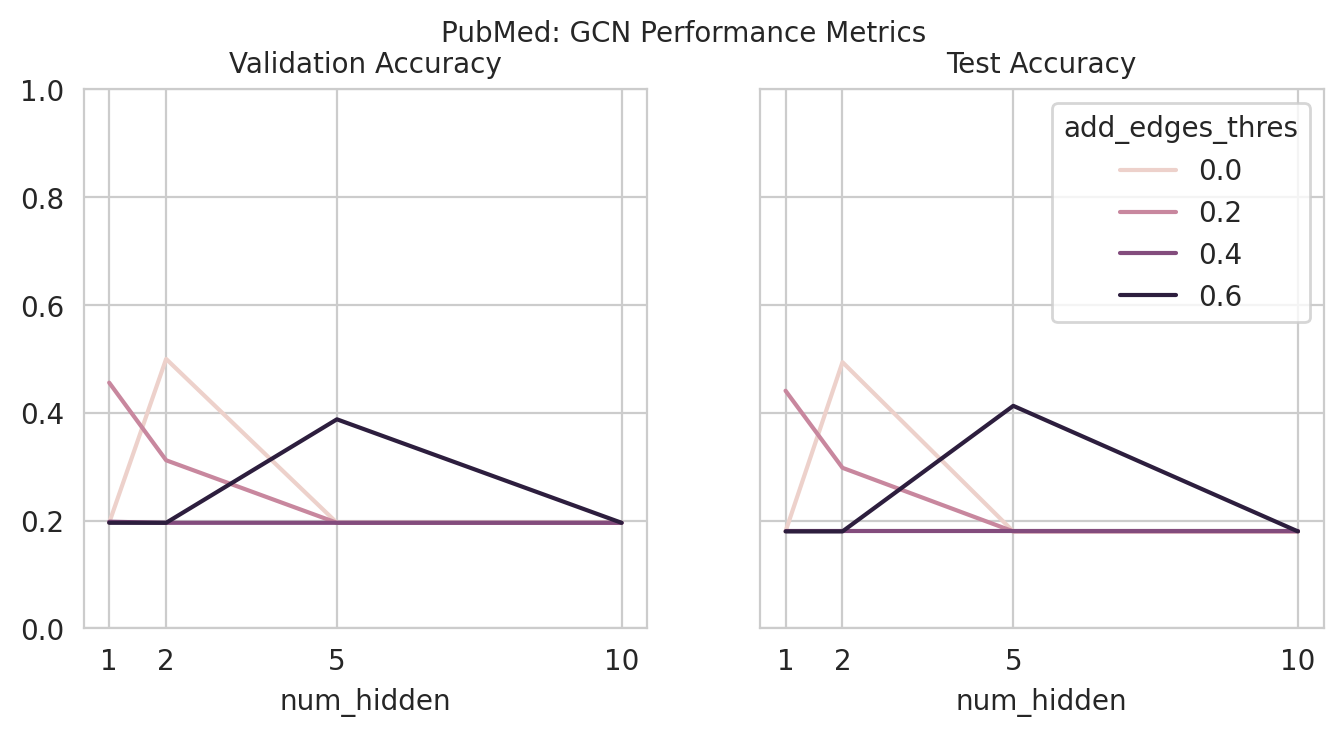
\includegraphics[scale=0.45]{gcn_performance.png}
    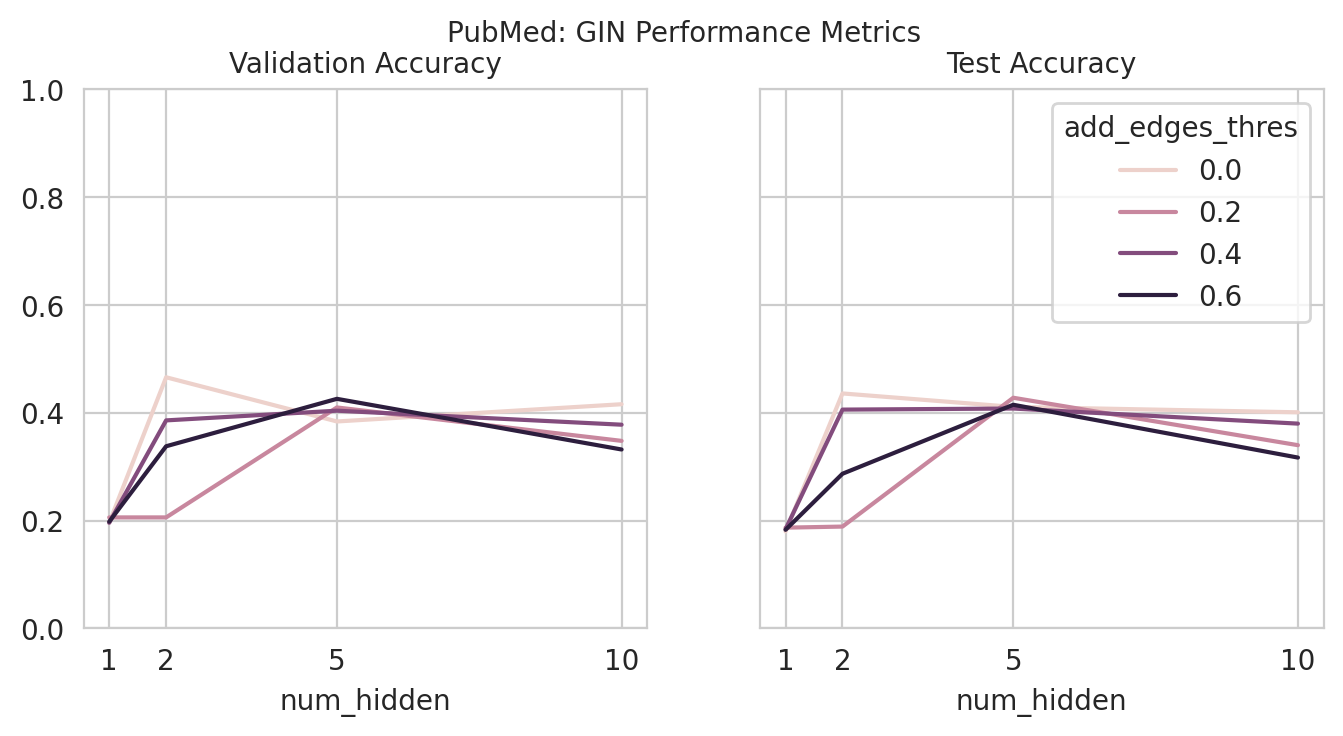
\includegraphics[scale=0.45]{gin_performance.png}
    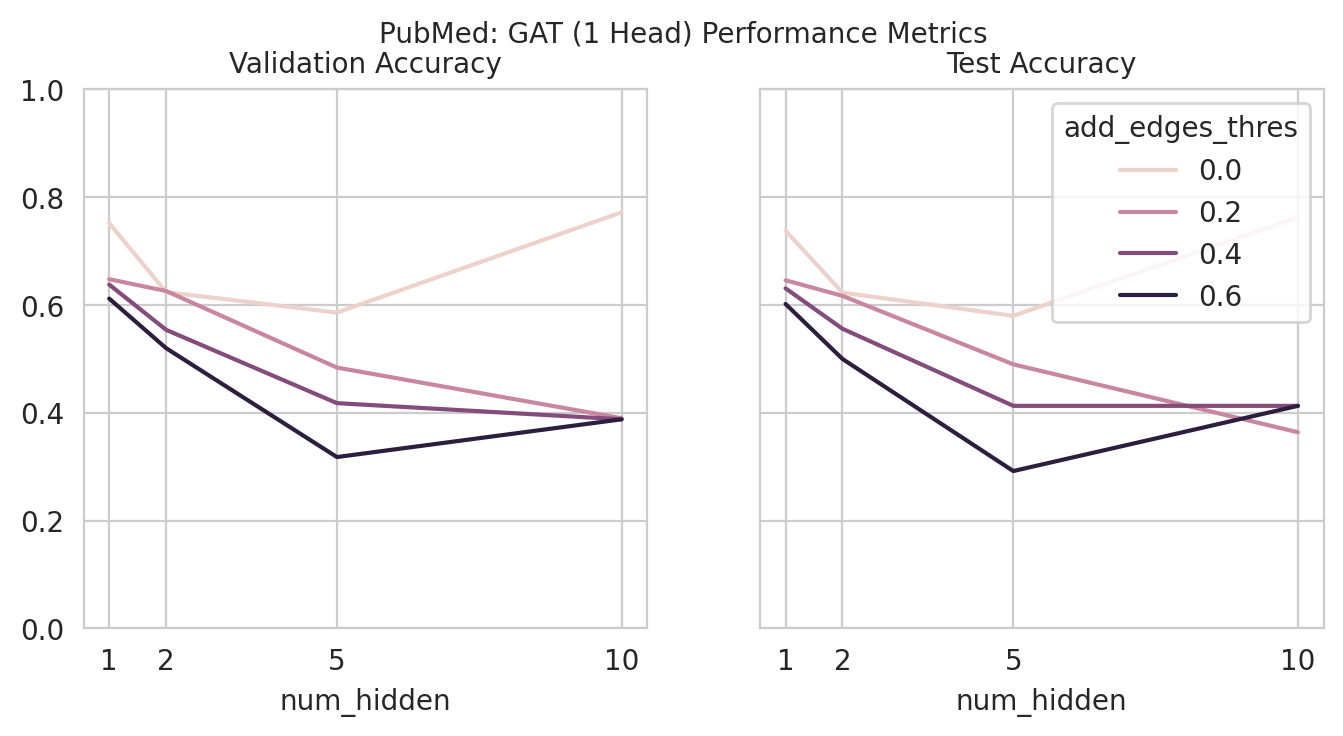
\includegraphics[scale=0.45]{gat_1_performance.png}
    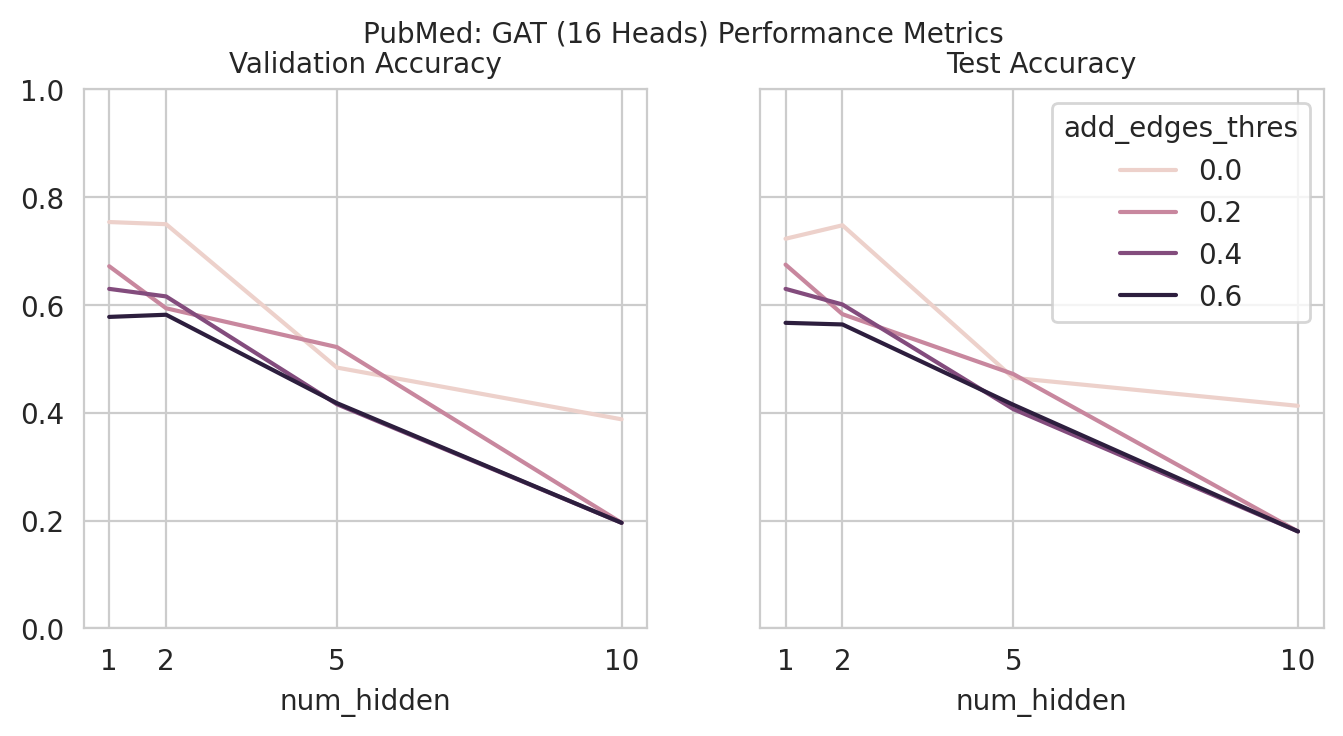
\includegraphics[scale=0.45]{gat_16_performance.png}
    \caption{PubMed performance metrics. Validation and test accuracy trends are displayed as a function of the number of hidden layers, colored by the number of edges randomly added to the input graph.}
    \label{fig:performance}
\end{figure}

\begin{figure}[h]
    \centering
    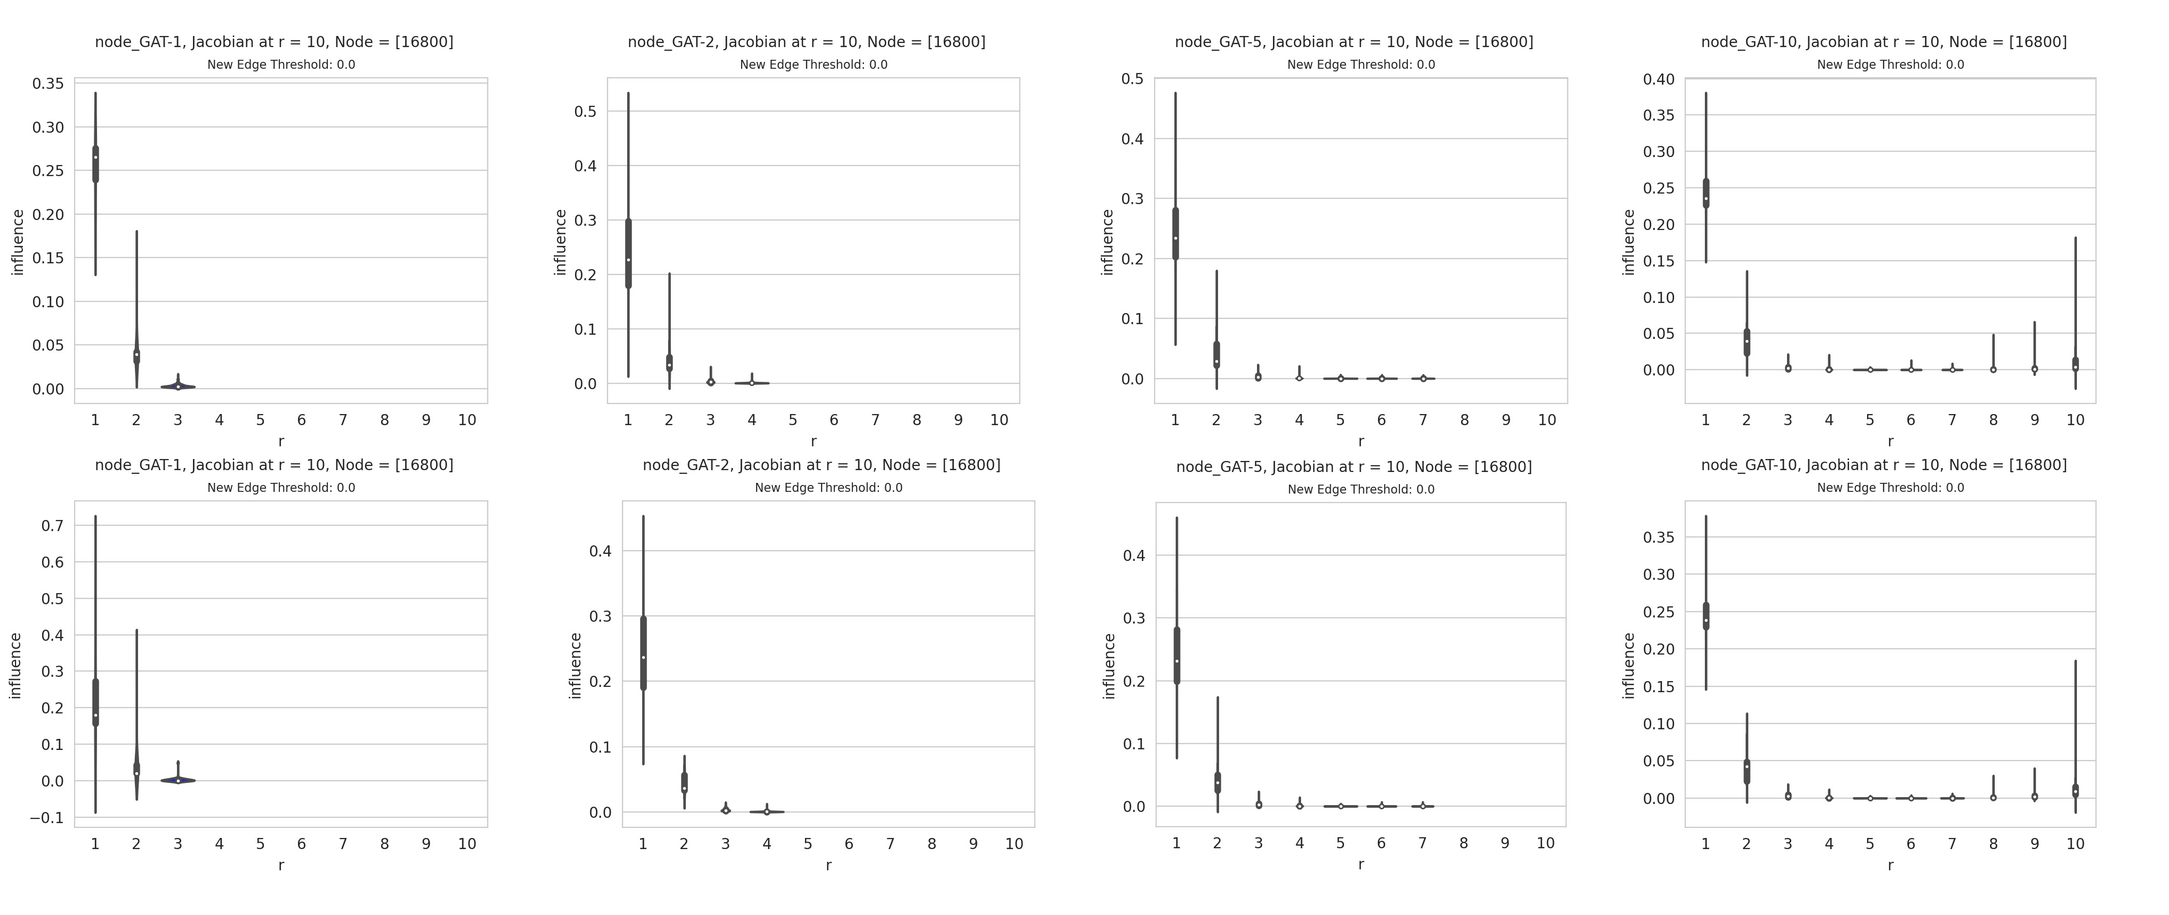
\includegraphics[scale=0.33, angle=90]{jacobians.png}
    \caption{An example of neighborhood influence distributions. Viewed sideways, the top row consists of distributions of the Jacobian embeddings from the single-headed GAT, for 1, 2, 5, to 10 hidden layers (left to right), with no data augmentation. The bottom row show the distributions for the multi-head GAT.}
    \label{fig:jacobian}
\end{figure}

\begin{figure}[h]
    \centering
    \includegraphics[scale=0.4]{node_GIN_10h_0.0.png}
    \includegraphics[scale=0.4]{node_GIN_10h_0.2.png}
    \includegraphics[scale=0.4]{node_GIN_10h_0.4.png}
    \includegraphics[scale=0.4]{node_GIN_10h_0.6.png}
    \caption{An example of exploding Dirichlet energy values of a 10-hidden layer GIN.}
    \label{fig:energy}
\end{figure}

\begin{figure}[h]
    \centering
    \includegraphics[scale=0.4]{node_GIN_10h_0.0_r.png}
    \includegraphics[scale=0.4]{node_GIN_10h_0.2_r.png}
    \includegraphics[scale=0.4]{node_GIN_10h_0.4_r.png}
    \includegraphics[scale=0.4]{node_GIN_10h_0.6_r.png}
    \caption{An example of exploding Dirichlet energy values of a 10-hidden layer GIN.}
    \label{fig:rayleigh}
\end{figure}


\end{document}
